% Copyright 2004 by Till Tantau <tantau@users.sourceforge.net>.
%
% In principle, this file can be redistributed and/or modified under
% the terms of the GNU Public License, version 2.
%
% However, this file is supposed to be a template to be modified
% for your own needs. For this reason, if you use this file as a
% template and not specifically distribute it as part of a another
% package/program, I grant the extra permission to freely copy and
% modify this file as you see fit and even to delete this copyright
% notice. 

\documentclass{beamer}

% There are many different themes available for Beamer. A comprehensive
% list with examples is given here:
% http://deic.uab.es/~iblanes/beamer_gallery/index_by_theme.html
% You can uncomment the themes below if you would like to use a different
% one:
%\usetheme{AnnArbor}
\usetheme{Antibes}%talvez
%\usetheme{Bergen}
%\usetheme{Berkeley}%talvez
%\usetheme{Berlin}
%\usetheme{Boadilla}
%\usetheme{boxes}
%\usetheme{CambridgeUS}
%\usetheme{Copenhagen}
%\usetheme{Darmstadt}
%\usetheme{default}
%\usetheme{Frankfurt}%talvez
%\usetheme{Goettingen}
%\usetheme{Hannover}
%\usetheme{Ilmenau}
%\usetheme{JuanLesPins}
%\usetheme{Luebeck}
%\usetheme{Madrid}
%\usetheme{Malmoe}
%\usetheme{Marburg}
%\usetheme{Montpellier}
%\usetheme{PaloAlto}%bomtema
%\usetheme{Pittsburgh}
%\usetheme{Rochester}
%\usetheme{Singapore}
%\usetheme{Szeged}
%\usetheme{Warsaw}

%\usepackage[brazil]{babel}
\usepackage[utf8]{inputenc}
\usepackage[brazil]{babel}
%\usepackage[latin1]{inputenc}
\usepackage{lmodern}
\usepackage{setspace}
\usepackage{verbatim}

% \usepackage{latex8}
\usepackage{subfloat}


\usepackage{algorithm}
\usepackage{algorithmic}
%\usepackage{times}
%\usepackage{amsmath}
%\usepackage{amssymb}
%\usepackage{setspace}
%\usepackage{graphicx}
%\usepackage{indentfirst}
%\usepackage{url}


\title{Seleção de Atributos \\via  Informação Estatística}

% A subtitle is optional and this may be deleted
%\subtitle{Optional Subtitle}

\author{Celio Henrique Nogueira Larcher Junior}
% - Give the names in the same order as the appear in the paper.
% - Use the \inst{?} command only if the authors have different
%   affiliation.

\institute[Laboratório Nacional de Computação Científica] % (optional, but mostly needed)
{
  Laboratório Nacional de Computação Científica
  %\and
  %\inst{2}%
  %Department of Theoretical Philosophy\\
  %University of Elsewhere
  }
% - Use the \inst command only if there are several affiliations.
% - Keep it simple, no one is interested in your street address.

\date{Petrópolis, 2017}
% - Either use conference name or its abbreviation.
% - Not really informative to the audience, more for people (including
%   yourself) who are reading the slides online

\subject{Ci\^encia da Computa\c{c}~ao}
% This is only inserted into the PDF information catalog. Can be left
% out. 

% If you have a file called "university-logo-filename.xxx", where xxx
% is a graphic format that can be processed by latex or pdflatex,
% resp., then you can add a logo as follows:

%\pgfdeclareimage[height=0.5cm]{university-logo}{figuras/university-logo-ufjf.png}
%\logo{\pgfuseimage{university-logo}}

% Delete this, if you do not want the table of contents to pop up at
% the beginning of each subsection:

% Let's get started
\begin{document}

\begin{frame}
  \titlepage
\end{frame}

\begin{frame}{Agenda}
\footnotesize
  \tableofcontents
  % You might wish to add the option [pausesections]
\end{frame}


\AtBeginSection[]
{
\begin{footnotesize}
  \begin{frame}<beamer>{Agenda}
    \tableofcontents[currentsection,currentsubsection]
  \end{frame}
  \end{footnotesize}
}

% Section and subsections will appear in the presentation overview
% and table of contents.


\section{Problema de Seleção de Atributos}

\begin{frame}{Introdução}
	\begin{itemize}
		\item Técnicas para seleção de atributos é a denominação de um grupo de técnicas que buscam extrair subconjuntos de atributos significativos da base de dados
		\item A seleção de atributos é uma operação importante no contexto de aprendizado de máquina:
		\begin{itemize}
			\item Permite a simplificação de modelos
			\item Diminui o tempo de treinamento
			\item Ameniza a ``maldição da dimensionalidade''
			\item Reduz o problema de \textit{overfitting}
		\end{itemize}
	\end{itemize}
\end{frame}


\begin{frame}{Definição}
	\begin{itemize}
		\item Dado uma base de dados formada pelo conjunto de atributos $S$, tem-se como objetivo encontrar um subconjunto $K \subseteq S$ suficientemente representativo:
		\begin{itemize}
			\item $|K|$ deve ser o menor possível
			\item Os atributos de $K$ devem ser capazes de conter informação semelhante ao visto em $S$
		\end{itemize}
		\item Em particular para classificação/regressão espera-se que $K$ tenha tanta informação sobre a saída $C$ quanto $S$
	\end{itemize}
\end{frame}



\section{Informação Estatística aplicada a Seleção de Atributos}


\begin{frame}{Critério da máxima dependência}
	\begin{itemize}
		\item A aplicação de informação mútua a um conjunto de atributos pode ser um bom indicativo da adequabilidade dos mesmos:
		$$I(K;C)=I(\{F_1,F_2,\dots,F_{|K|}\};C)$$
		\item Desta forma, tem-se um indicativo do quanto o conjunto de atributos tem de informação em comum com os valores de saída ($C$).
	\end{itemize}
\end{frame}

\begin{frame}{Critério da máxima dependência - Problemas}
	\begin{itemize}
		\item Porém o número de atributos não é penalizado, não sendo desencorajada a escolha de atributos redundantes.	
		\item Além disto, calcular a informação mútua de um conjunto de atributos pode ser custoso.
		\item Necessária a aplicação da regra da cadeia, ou outro mecanismo que o valha.
		$$I(K;C)=\sum_{i=1}^{|K|} I(F_i; C| F_{i-1}, F_{i-2}, \dots, F_{1})=I(K)+I(C)-I(K,C)$$
		\item Complexidade cresce proporcionalmente ao produto das dimensão dos espaços de atributos (produto cartesiano)
%		\item Comum a utilização de aproximações para a informação mútua dos subconjuntos.
	\end{itemize}
\end{frame}

%\subsection{Multivariada}

\begin{frame}{mRMR - min-Redundancy Max-Relevance}
	\begin{itemize}
		\item Uma opção menos custosa é o método mRMR:
		$$I(F_j;C)- \frac{1}{|K|} \sum_{F_i \in K} I(F_j;F_i)$$
		\item Pondera a informação ganha pela adição de um novo atributo com a redundância para os atributos já selecionados no conjunto $K$.
		\item Ainda possui complexidade considerável (proporcional ao número de atributos já selecionado).
	\end{itemize}
\end{frame}



\begin{frame}{Ganho de informação}
	\begin{itemize}
		\item Como uma alternativa de custo consideravelmente mais baixo tem-se a métrica do ganho de informação:
		$$G_i=I(C)-I(C|F_i)=I(C;F_i)$$

		\item O ganho de informação é dado pela diferença entre a entropia para a classe de saída e a entropia ao se utilizar o atributo $F_i$.
		\item Não há qualquer consideração em relação aos atributos já selecionados.

%\noindent onde:		
%		
%$I(C)=-\sum_{c_j \in C} p(c_j) \log p(c_j)$
%$I(C|F_i)=-\sum_{f_i \in F_i} p(f_i) \sum_{c_j \in C} p(c_j |f_i) \log p(c_j|f_i)$

	\end{itemize}
\end{frame}


\begin{frame}{Informação normalizada}
	\begin{itemize}
		\item Ainda outra alternativa semelhante é a a informação normalizada:
		$$R_i=\frac{I(C)-I(C|F_i)}{I(F_i)}=\frac{I(C;F_i)}{I(F_i)}$$

		\item Considera atributos de menor informação própria como mais relevantes para seleção.

%\noindent onde 
%		
%$I(C)=-\sum_{c_j \in C} p(c_j) \log p(c_j)$
%$I(C|F_i)=-\sum_{f_i \in F_i} p(f_i) \sum_{c_j \in C} p(c_j |f_i) \log p(c_j|f_i)$
%$I(F_i)=-\sum_{f_i \in F_i} p(f_i) \log p(f_i)$

	\end{itemize}
\end{frame}


\begin{frame}{Exploração do espaço de busca}
	\begin{itemize}
		\item Outro ponto a ser definido além das métricas para seleção são os métodos de exploração.
		\item Espaço total para exploração é exponencial ($2^{|S|}$)
		\item Opções para exploração:
		\begin{itemize}
			\item Exploração completa (caro)
			\item Procedimento guloso (sub-ótimo)
			\item Procedimentos adaptativos (metaheurísticas)
		\end{itemize}
	\end{itemize}
\end{frame}




\section{Experimentos}

\begin{frame}{Configuração}
	\begin{itemize}
		\item Para realização dos experimentos foi selecionado a base de dados \textit{Young People Survey} do repositório \textit{Kaggle}
		\item A base consiste de 150 atributos e 1010 registros
		\item Foi implementado um procedimento de seleção guloso para seleção dos atributos
		\item Para avaliação do processo de classificação utilizou-se o algoritmo SVM
	\end{itemize}
\end{frame}


\begin{frame}
	\begin{figure}[ht]
		\begin{center}
 	 	  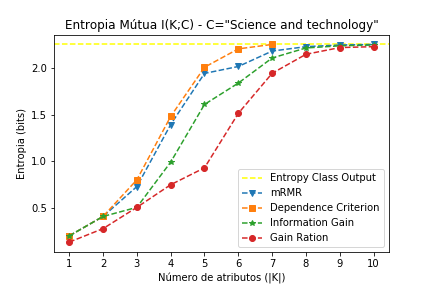
\includegraphics[scale=0.7]{figuras/Entropy_Science_and_technology.png}	
		  \label{fig:fluxogramaAG}		
%		  \caption{Tempo de processamento}	  
		\end{center}
	\end{figure}
\end{frame}

\begin{frame}
	\begin{figure}[ht]
		\begin{center}
 	 	  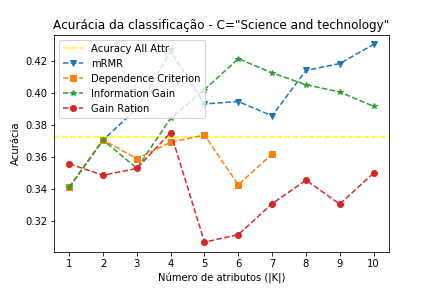
\includegraphics[scale=0.7]{figuras/Acuracy_Science_and_technology.png}	
		  \label{fig:fluxogramaAG}		
%		  \caption{Tempo de processamento}	  
		\end{center}
	\end{figure}
\end{frame}



\begin{frame}
	\begin{figure}[ht]
		\begin{center}
 	 	  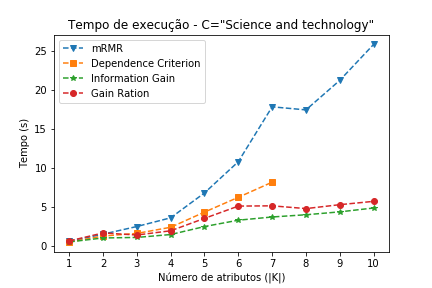
\includegraphics[scale=0.7]{figuras/Time_Science_and_technology.png}	
		  \label{fig:fluxogramaAG}		
%		  \caption{Tempo de processamento}	  
		\end{center}
	\end{figure}
\end{frame}

\begin{frame}{Atributos selecionados}
	\begin{itemize}
		\item Mrmr: [PC, Physics, Documentary, Cars, Branded clothing, Gender, Sci-fi, Adrenaline sports, Daily events, Funniness] 
\item Dependence Criterion: [PC, Physics, Cars, Horror, Branded clothing, Spending on healthy eating, Pets] 
\item Information Gain: [PC, Physics, Gender, Cars, Documentary, Height, Sci-fi, Spending on gadgets, Life struggles, Action] 
\item Gain Ration: [Gender, Physics, PC, Height, Weight, Cars, Documentary, Sci-fi, Spending on gadgets, Western] 
	\end{itemize}
\end{frame}

\begin{frame}
	\begin{figure}[ht]
		\begin{center}
 	 	  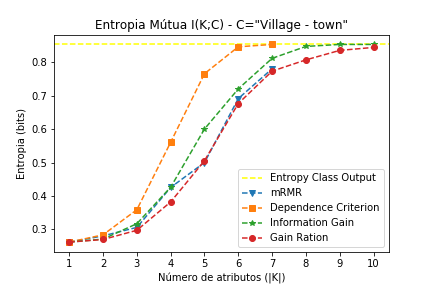
\includegraphics[scale=0.7]{figuras/Entropy_Village-town.png}	
		  \label{fig:fluxogramaAG}		
%		  \caption{Tempo de processamento}	  
		\end{center}
	\end{figure}
\end{frame}

\begin{frame}
	\begin{figure}[ht]
		\begin{center}
 	 	  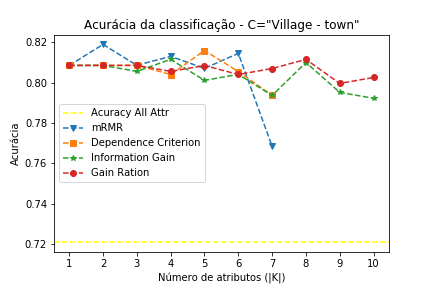
\includegraphics[scale=0.7]{figuras/Acuracy_Village-town.png}	
		  \label{fig:fluxogramaAG}		
%		  \caption{Tempo de processamento}	  
		\end{center}
	\end{figure}
\end{frame}



\begin{frame}
	\begin{figure}[ht]
		\begin{center}
 	 	  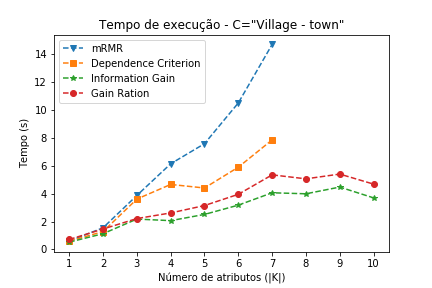
\includegraphics[scale=0.7]{figuras/Time_Village-town.png}	
		  \label{fig:fluxogramaAG}		
%		  \caption{Tempo de processamento}	  
		\end{center}
	\end{figure}
\end{frame}


\begin{frame}{Atributos selecionados}
	\begin{itemize}
		\item Mrmr: [House - block of flats, Friends versus money, Punctuality, Geography, Only child, Punk, Height] 
		\item Dependence Criterion: [House - block of flats, Punk, Passive sport, War, Rats, Biology, Public speaking] 
		\item Information Gain: [House - block of flats, Religion, Gardening, Friends versus money, Number of siblings, Storm, Countryside - outdoors, Punk, Final judgement, God] 
		\item Gain Ration: [House - block of flats, Movies, Gardening, Religion, Number of siblings, Storm, Friends versus money, Punctuality, Countryside - outdoors, Personality] 
	\end{itemize}
\end{frame}

\section{Comentários}

\begin{frame}{Sobre o experimento}
	\begin{itemize}
		\item A informação mútua não é diretamente proporcional à acurácia obtida (dependente da capacidade de generalização/representação da técnica de aprendizado)
%		\item A validação cruzada pode privar o algoritmo de aprendizado de determinadas amostras relevantes
		\item Espaço amostral pequeno: 1010 registros X $\approx 5^{150}$ possibilidades)
		\item Tempo de execução obtido não é absoluto (carece de otimizações)
		\item Método de seleção guloso não garante a melhor escolha possível para cada métrica
	\end{itemize}
\end{frame}

\begin{frame}{Sobre as técnicas}
	\begin{itemize}
		\item Mais atributos podem levar a um modelo mais complexo, mas de menor acurácia
		\item A possibilidade de redução para a dimensionalidade é substancial para ambas as tarefas de classificação analisadas
		\item A técnica máxima dependência possui uma convergência mais rápida em relação a entropia, porém com desempenho inferior para acurácia dos modelos gerados
		\item A técnica mRMR foi a que demonstrou um melhor balanço entre acurácia e entropia, porém foi a de maior tempo de execução
		\item As técnicas de Ganho de Informação e Informação Normalizada não apresentam comportamento constante para acurácia, mas Ganho de Informação tem maior crescimento da entropia
	\end{itemize}
\end{frame}




\section{Refer\^encias}

% All of the following is optional and typically not needed. 
\appendix
\section<presentation>*{\appendixname}
\subsection<presentation>*{Refer\^encias}

\begin{frame}[allowframebreaks]
\scriptsize
  \frametitle<presentation>{Refer\^encias}
    
  \begin{thebibliography}{10}
  
  \beamertemplatearticlebibitems
  % Followed by interesting articles. Keep the list short.     
	
	 \bibitem{Bonev10}
	Bonev, B. I. (2010). 
	\newblock{Feature Selection Based on Information Theory. \em PHD Thesis.}
	
	
	\bibitem{Duch10}
	 Duch, W., Biesiada, J., Winiarski, T., Grudziński, K., Grabczewski, K. (2003). 
	\newblock{Feature Selection Based on Information Theory
Filters. \em Neural Networks and Soft Computing: Proceedings of the Sixth International Conference on Neural Networks and Soft Computing, Zakopane, Poland, June 11--15, 2002.}
	

	 \bibitem{Mohammad06}
	Kaggle - Young People Survey. 
	\newblock{https://www.kaggle.com/miroslavsabo/young-people-survey}


	\bibitem{Vergara14}
	Vergara, J. , Estévez, P. (2014). 
	\newblock{A review of feature selection methods based on mutual information. \em Neural Computing and Applications.}
	
  \end{thebibliography}
\end{frame}

\begin{frame}
	\begin{center}
	
	\Huge{Obrigado pela atenção!}
	
	\end{center}
\end{frame}

\end{document}
